% Filename: cap03@notas_de_aula.tex
% This code is part of 'Notas de aula não oficiais de MS650 e F620'
% 
% Description: This file correspond to part of the textbook using in the course.
% 
% Created: 01.09.12 10:44:19 AM
% Last Change: 01.09.12 10:44:19 AM
% 
% Authors:
% - Raniere Silva, r.gaia.cs@gmail.com
% 
% Copyright (c) 2012, Raniere Silva. All rights reserved.
% 
% This work is licensed under the Creative Commons Attribution-NonCommercial-NoDerivs 3.0 Unported License. To view a copy of this license, visit http://creativecommons.org/licenses/by-nc-nd/3.0/.
%
% This work is distributed in the hope that it will be useful, but WITHOUT ANY WARRANTY; without even the implied warranty of MERCHANTABILITY or FITNESS FOR A PARTICULAR PURPOSE.
%
\chapter{Noções Básicas de Teoria das Distribuições}
\section{Motivações}
Vamos considerar a função $\phi_N(x)$ definida como
\begin{dmath*}
  \phi_N(x) = \begin{cases}
    N / 2, & \lvert x \rvert \leq 1 / N, \\
    0 & \lvert x \rvert > 1 / N.
  \end{cases}
\end{dmath*}
\begin{figure}[htb]
  \centering
  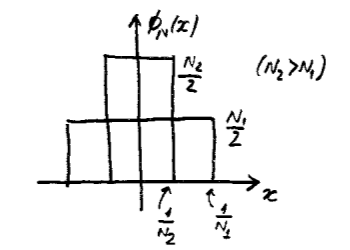
\includegraphics{figuras/08-0}
\end{figure}
% TODO Inserir número da página.
A série de Fourier dessa função já foi calculada (página ???, onde $a = 1 / N$)
tomando $L > 1 / N$, ou seja,
\begin{dmath*}
  \phi_N(x) = \frac{1}{2 L} + \sum_{n = 1}^{\infty} \left( \frac{N}{n \pi}
  \sin\left( \frac{n \pi}{N L} \right) \right) \cos\left( \frac{n \pi x}{L}
  \right).
\end{dmath*}

É fácil notarmos que à medida que aumentamos $N$, a função $\phi_N(x)$ fica cada
vez mais concentrada em torno de $x = 0$. A idéia intuitiva é que, para $N \to
\infty$, devemos ter
\begin{dmath*}
  \lim_{N \to \infty} \phi_N(x) = \begin{cases}
    +\infty, & x = 0, \\
    0, & x \neq 0.
  \end{cases}
\end{dmath*}
O problema, porém, é que não há sentido em definirmos uma função cujo valor em
um ponto seja $+\infty$. Também não temos como contornar esse problema
trabalhando com a série de Fourier pois ela não converge para $N \to \infty$, de
fato:
\begin{dmath*}
  \lim_{N \to \infty} \sum_{n = 1}^{\infty} \left( \frac{N}{n \pi} \sin\left(
  \frac{n \pi}{N L} \right) \right) \cos \left( \frac{n \pi x}{L} \right) =
  \sum_{n = 1}^{\infty} \frac{1}{L} \cos\left( \frac{n \pi x}{L} \right)
\end{dmath*}
que evidentemente não converge.

% TODO Inserir número da página.
Por outro lado, do teorema referente à integração da série de Fourier (página
???) sabemos que se $\phi_N(x)$ é contínua por partes, valoe a identidade
relacionada com a integração da série independentemente da série convergir ou
não. De fato:
\begin{dgroup*}
  \begin{dmath*}
    \int_{-L}^L \phi_N(x) \vi{x} = \int_{-1/N}^{1/N} N / 2 \vi{x}
    = (N / 2) (2 / N)
    = 1,
  \end{dmath*}
  \begin{dmath*}
    \int_{-L}^L \left( \frac{1}{2 L} + \sum_{n = 1}^{\infty}
    \frac{N}{n \pi} \sin\left( \frac{n \pi}{N L} \right) \cos\left(
    \frac{n \pi x}{L} \right) \right) = \frac{1}{2 L} 2 L + \sum_{n =
    1}^{\infty} \frac{N}{n \pi} \sin\left( \frac{n \pi}{N L} \right)
    \frac{L}{n \pi} \left. \sin\left( \frac{n \pi x}{L} \right) \right|_{-L}^L
    = \frac{1}{2 L} 2 L + \sum_{n = 1}^{\infty} \frac{N}{n \pi} \sin\left(
    \frac{n \pi}{N L} \right) \frac{L}{n \pi} 0
    = 1,
  \end{dmath*}
\end{dgroup*}
ou seja,
\begin{dmath*}
  \int_{-L}^L \phi_N(x) \vi{x} = \int_{-L}^L \left( \frac{1}{2 L} + \sum_{n =
  1}^{\infty} \frac{N}{n \pi} \sin\left( \frac{n \pi}{n L} \right) \cos\left(
  \frac{n \pi x}{L} \right) \right)
  = 1 \condition{$\forall N$}
\end{dmath*}
de modo que
\begin{dmath*}
  \lim_{N \to \infty} \int_{-L}^L \phi_N(x) \vi{x} = 1
\end{dmath*}
embora não exista $\lim_{N \to \infty} \phi_N(x)$.

Na verdade, podemos ir mais além. Seja $f(x)$ uma função que por enquanto basta
supor que possa ser representada por uma série de Fourier. Então:
\begin{dmath*}
  \int_{-L}^L f(x) \phi_N(x) \vi{x} = \int_{-L}^L \left( \frac{1}{2 L} + \sum_{n
  = 1}^{\infty} \frac{N}{n \pi} \sin\left( \frac{n \pi}{N L} \right) \cos\left(
  \frac{n \pi x}{L} \right)\right) f(x) \vi{x}
  = \frac{1}{2} \left[ \frac{1}{L} \int_{-L}^L f(x) \vi{x} \right] + \sum_{n =
  1}^{\infty} \frac{N L}{n \pi} \sin\left( \frac{n \pi}{N L} \right) \left[
  \frac{1}{L} \int_{-L}^L f(x) \cos\left( \frac{n \pi x}{L} \right) \right]
  = \frac{a_0}{2} + \sum_{n = 1}^{\infty} a_n \frac{N L}{n \pi} \sin\left(
  \frac{n \pi}{N L} \right)
\end{dmath*}
onde $a_0$ e $a_n$ são os coeficientes de Fourier de $f(x)$,
\begin{dmath*}
  f(x) = \frac{a_0}{2} + \sum_{n = 1}^{\infty} \left( a_n \cos\left(
  \frac{n \pi x}{L} \right) + b_n \sin\left( \frac{n \pi x}{L} \right) \right).
\end{dmath*}
Tomando $N \to \infty$,
\begin{dmath*}
  \lim_{N \to \infty} \int_{-L}^L f(x) \phi_N(x) \vi{x} = \frac{a_0}{2} +
  \sum_{n = 1}^{\infty} a_n
\end{dmath*}
que nada mais é do que $f(0)$,
\begin{dmath*}
  \lim_{N \to \infty} \int_{-L}^L f(x) \phi_N(x) \vi{x} = f(0)
\end{dmath*}
muito embora $\nexists \lim_{N \to \infty} \phi_N(x)$.

Na verdade, nós já nos deparamos com uma sitação análoga. Do Teorema de Fourier
e da expressão para o núcleo de Dirichlet, temos (considerando um período $T = 2
L$)
\begin{dmath*}
  f(x) = \lim_{N \to \infty} \int_{-L}^L f(\epsilon) D_N(\epsilon - x)
  \vi{\epsilon}
\end{dmath*}
onde
\begin{dmath*}
  D_N(x) = \frac{1}{2 L} \frac{\sin(N + 1/2) \pi x / L}{\sin(\pi x / (2 L))}.
\end{dmath*}
Como podemos ver $\nexists \lim_{N \to \infty} D_N(x)$ e mesmo assim
\begin{dgroup*}
  \begin{dmath*}
    \lim_{N \to \infty} \int_{-L}^L f(x) D_N(x) \vi{x} = f(0),
  \end{dmath*}
  \begin{dmath*}
    \lim_{N \to \infty} \int_{-L}^L D_N(x) \vi{x} = 1.
  \end{dmath*}
\end{dgroup*}
Temos, portanto, sequências que não convergem no sentido usual mas que, quando
tomadas dentro de uma integral com uma função $f(x)$, convergem para o mesmo
resultado, no caso $f(0$. Podemos pensar que essas sequências convergem (em um
outro sentido) para uma ``função'' $\delta(x)$ tal que $\int_{-L}^L \delta(x)
f(x) \vi{x} = f(0)$. Essa é a idéia que usaremos. Além disso, para aumentar a
classe de sequências que consideramos, vamos tomar $L \to \infty$, e para
assegurar que as integrais estejam bem definidas, vamos restringir o conjunto
das funções $f(x)$ que tomaremos nas integrais.

\section{Função Delta de Dirac}
\begin{defi}
  Uma função-teste é uma função infinitamente diferenciável tal que ela é
  identicamente nula fora de um intervalo finito $(a, b)$. Denotaremos o
  conjunto das funções-teste por $\mathcal{D}(R)$.
\end{defi}
\begin{exem}
  Um exemplo clássico de função-teste é
  \begin{dmath*}
    f(x) = \begin{cases}
      \exp(-1 / (1 - x^2), & \lvert x \rvert < 1, \\
      0, & \lvert x \rvert 1 \geq 1.
    \end{cases}
  \end{dmath*}
  Outros exemplos seguem quando notamos que se $f(x)$ é uma função-teste e
  $Q(x)$ é uma função infinitamente diferenciável, então $Q(x) f(x)$ é uma
  função-teste.
\end{exem}
\begin{defi}
  Uma sequência delta é uma sequência $\left\{ \phi_N(x) \right\}$ satisfazendo
  \begin{dmath*}
    \lim_{n \to \infty} \int_{-\infty}^{+\infty} \phi_n(x) \vi{x} = 1
  \end{dmath*}
  e, para $f(x) \in \mathcal{D}(R)$,
  \begin{dmath*}
    \lim_{n \to \infty} \int_{-\infty}^{+\infty} \phi_n(x) f(x) \vi{x} = f(0).
  \end{dmath*}
  Definimos a função delta de Dirac como sendo o limite de uma sequência delta,
  onde esse limite é interpretado no sentido de
  \begin{dmath*}
    \int_{-\infty}^{+\infty} \delta(x) f(x) \vi{x} = \lim_{n \to \infty}
    \int_{-\infty}^{+\infty} \phi_n(x) f(x) \vi{x}.
  \end{dmath*}
  Assim sendo, a função delta de Dirac satisfaz
  \begin{dmath*}
    \int_{-\infty}^{+\infty} \phi_(x) f(x) \vi{x} = f(0).
  \end{dmath*}
  Evidentemente $\delta(x)$ não é uma ``função'' no sentido usual. Ela é o que
  chamamos uma ``função generalizada'' ou ``distribuição''.
\end{defi}
\begin{exem}
  Exemplos de sequência delta, além daquelas da seção anterior, são:
  \begin{enumerate}
    \item $\phi_n(x) = (n / \pi) (1 / (1 + n^2 x^2))$,
    \item $\phi_n(x) = (n / \sqrt{\pi}) \exp(-n^2 x^2)$,
    \item $\phi_n(x) = 1 / (n \pi) (\sin^2(n x) / x^2)$,
    \item $\phi_n(x) = n J_n(n (1 + x))$,
    \item $\phi_n(x) = n \exp(-n x^2) L_k(2 n x)$,
  \end{enumerate}
  onde $J_n(x)$ é a função de Bessel de ordem $n$ e $L_k(x)$ é o polinômio de
  Laguere de ordem $k$ (arbitrário).
\end{exem}

Podemos ainda definir a função delta transladada $\delta(x - a)$. Nesse caso:
\begin{dmath*}
  \int_{-\infty}^{+\infty} \delta(x - a) f(x) \vi{x} = f(a).
\end{dmath*}
Para vermos isso usamos a definição via sequência delta:
\begin{dmath*}
  \int_{-\infty}^{+\infty} \delta(x - a) f(x) \vi{x} = \lim_{n \to \infty}
  \int_{-\infty}^{+\infty} \phi_n(x - a) f(x) \vi{x}
  = \lim_{n \to \infty} \int_{-\infty}^{+\infty} \phi_n(y) f(y + a) \vi{y}
  = \int_{-\infty}^{+\infty} \delta(y) f(y + a) \vi{y}
  = f(a).
\end{dmath*}
Isso, aliás, mostra que podemos fazer mudanças de variáveis diretamente dentro
da integral com a função delta. Dessa forma podemos mostrar por exemplo, que
para $a \neq 0$
\begin{dmath*}
  \delta(a x) = \delta(x) / \lvert a \rvert.
\end{dmath*}
De fato, se $a > 0$:
\begin{dmath*}
  \int_{-\infty}^{+\infty} \delta(a x) f(x) \vi{x} = \int_{-\infty}^{+\infty}
  \delta(y) f(y / a) \frac{\vi{y}}{a}
  = \frac{f(0)}{a}
  = \int_{-\infty}^{+\infty} \frac{\delta(x)}{\lvert a \rvert} f(x) \vi{x}
\end{dmath*}
enquanto, se $a < 0$:
\begin{dmath*}
  \int_{-\infty}^{+\infty} \delta(a x) f(x) \vi{x} = \int_{+\infty}^{-\infty}
  \delta(y) f(y / a) \frac{\vi{y}}{a}
  = -\frac{f(0)}{a}
  = \int_{-\infty}^{+\infty} \frac{\delta(x)}{\lvert a \rvert} f(x) \vi{x}.
\end{dmath*}

Já com um pouco mais de engenhosidade, podemos mostrar que, para $a \neq 0$:
\begin{dmath*}
  \delta(x^2 - a^2) = \frac{1}{2 \lvert a \rvert} \left[ \delta(x + a) +
  \delta(x - a) \right].
\end{dmath*}
Para isso vamos considerar as funções-teste que são identicamente nulas fora do
intervalo $(-a , a)$. Vamos denotar esse conjunto por $\mathcal{D}(-a, a)$, de
mode que $\mathcal{D}(-a, a) \subset \mathcal{D}(R)$. Tomando $x^2  - a^2 = y$,
temos que para $x \geq 0$, $x = \sqrt{y - a^2}$, $y - a^2 \leq y < \infty$,
enquanto para $x \leq 0$, $x = -\sqrt{y + a^2}$, $-a^2 \leq y < \infty$. Logo
\begin{dmath*}
  \int_{-\infty}^{+\infty} \delta(x^2 - a^2) f(x) \vi{x} = \int_{-\infty}^0
  \delta(x^2 - a^2) f(x) \vi{x} + \int_0^{\infty} \delta(x^2 - a^2) f(x) \vi{x}
  = \int_{-\infty}^{-a^2} \delta(y) f(-\sqrt{y + a^2}) \frac{- \vi{y}}{2 \sqrt{y
  + a^2}} + \int_{-a^2}^{\infty} \delta(y) f(\sqrt{y + a^2})
  \frac{\vi{y}}{2 \sqrt{y + a^2}}
  = \frac{f(-\sqrt{a^2})}{2\sqrt{a^2}} + \frac{f(\sqrt{a^2})}{2 \sqrt{a^2}}
  = \frac{1}{2 \lvert a \rvert} \int_{-\infty}^{+\infty} \left[ \delta(x + a) +
  \delta(x - a) \right] f(x) \vi{x},
\end{dmath*}
onde usamos que $f(x) \in \mathcal{D}(-a, a)$. Portanto $\delta(x^2 - a^2)$ age
sobre $f \in \mathcal{D}(-a, a)$ de uma forma tal que é a mesma que $1 / (2
\lvert a \rvert) \left[ \delta(x + a) + \delta(x - a) \right]$ agindo sobre $f
\in \mathcal{D}(R)$.

Dentro do cálculo com a função delta, é natural procurarmos definir a derivada
$\delta'(a)$. Se $\left\{ \phi_n(x) \right\}$ é uma sequência delta, definimos
$\delta'(a)$ como a distribuição associada com as derivadas dessa sequência, ou
seja,
\begin{dmath*}
  \int_{-\infty}^{+\infty} \delta'(x) f(x) \vi{x} = \lim_{n \to \infty}
  \int_{-\infty}^{+\infty} \phi'_n(x) f(x) \vi{x},
\end{dmath*}
onde $f \in \mathcal{D}(R)$. Mas, integrando por partes
\begin{dmath*}
  \int_{-\infty}^{+\infty} \phi'_n(x) f(x0 \vi{x} = \left. \phi_n(x) f(x)
  \right|_{-\infty}^{+\infty} - \int_{-\infty}^{+\infty} \phi_n(x) f'(x) \vi{x}
\end{dmath*}
e como $f(x) \equiv 0$ para $x \notin (a, b)$, de modo que $\lim_{x \to
\pm\infty} f(x) = 0$,
\begin{dmath*}
  \left. \phi_n(x) f(x) \right|_{-\infty}^{+\infty} = 0
\end{dmath*}
e portanto
\begin{dmath*}
  lim_{n \to \infty} \int_{-\infty}^{+\infty} \phi'_n(x) f(x) \vi{x} = -\lim_{n
  \to \infty} \int_{-\infty}^{+\infty} \phi_n(x) f'(x) \vi{x}
  = -\int_{-\infty}^{+\infty} \delta(x) f'(x) \vi{x}
  = -f'(0).
\end{dmath*}
Portanto,
\begin{dmath*}
  \int_{-\infty}^{+\infty} \delta'(x) f(x) \vi{x} = -f'(0).
\end{dmath*}

A derivada $n$-ésima $d^{(n)}(x)$ é definida de forma análoga. Repetindo os
passos aacima, lembranddo que $f^{(k)}(x) \equiv 0$ para $x \notin (a, b)$ e $k
= 0, 1, 2, \ldots$, segue que
\begin{dmath*}
  \int_{-\infty}^{+\infty} \delta^{(n)}(x) f(x) \vi{x} = (-1)^n f^{(n)}(0).
\end{dmath*}

Podemos ainda nos perguntar pela primiteva da função delta, ou seja, uma
distribuição $H(x)$ tal que $\delta(x) = H'(x)$. A definição natural é
\begin{dmath*}
  \int_{-\infty}^{+\infty} H(x) f(x) \vi{x} = \lim_{n \to \infty}
  \int_{-\infty}^{+\infty} \Phi_n(x) f(x) \vi{x}
\end{dmath*}
onde $\Phi_n(x)$ é uma primitiva de $\phi_n(x)$, por exemplo:
\begin{dmath*}
  \Phi_n(x) = \int_{-\infty}^x \phi_n(x)(\epsilon) \vi{\epsilon}.
\end{dmath*}
Com isso e trocando a ordem de integração
\begin{dmath*}
  \int_{-\infty}^{+\infty} \Phi_n(x) f(x) \vi{x} = \int_{-\infty}^{+\infty}
  \left[ \int_{-\infty}^x \phi_n(\epsilon) \vi{\epsilon} \right] f(x) \vi{x}
  = \int_{-\infty}^{+\infty} \left[ \int_{\epsilon}^{+\infty} f(x) \vi{x}
  \right] \phi_n(\epsilon) \vi{\epsilon}
\end{dmath*}
e como isso
\begin{dmath*}
  \lim_{n \to \infty} \int_{-\infty}^{+\infty} \Phi_n(x) f(x) \vi{x} = \lim_{n
  \to \infty} \int_{-\infty}^{+\infty} \phi_n(\epsilon) \left[
  \int_{\epsilon}^{+\infty} f(x) \vi{x} \right] \vi{\epsilon}
  = \int_{-\infty}^{+\infty} \delta(\epsilon) \left[ \int_{\epsilon}^{+\infty}
  f(x) \vi{x} \right] \vi{\epsilon}
  = \int_0 {\infty} f(x) \vi{x},
\end{dmath*}
ou seja,
\begin{dmath*}
  \int_{-\infty}^{+\infty} H(x) f(x) \vi{x} = \int_0^{\infty} f(x) \vi{x}
\end{dmath*}
de modo que
\begin{dmath*}
  H(x) = \begin{cases}
    1, & x > 0, \\
    0, & x < 0,
  \end{cases}
\end{dmath*}
que é a chamada função escada ou de Heaviside.

\begin{exem}
  As seguintes sequência convergem (no sentido de $\lim_{n \to \infty}
  \int_{-\infty}^{+\infty} \Phi_n(x) f(x) \vi{x} = \int_{-\infty}^{+\infty} H(x)
  f(x) \vi{x})$) para a função escada:
  \begin{itemize}
    \item $\Phi_n(x) = (1 / 2) \operatorname{erfc}(-n x) = (1 / \sqrt{\pi})
      \int_{-n x}^{\infty} \exp(-u^2) \vi{u}$,
    \item $\Phi_n(x) = (1 / 2) + (1 / \pi) \sin(n x) = (1 / \pi)
      \int_{-\infty}^{n x} \sin(u) / u \vi{u}$,
    \item $\Phi_n(x) = \exp(- \exp(n x))$.
  \end{itemize}
\end{exem}
